\chapter{Grundlagen der Elektronenstoßionisation}
\label{chap:ion}
Das grundlegende Prinzip auf dem die Ionisation in einem RIT und die massenspektrometrische Messung dieser Arbeit basieren ist die Elektronenstoßionisation von Atomen, Molekülen und Ionen. 
Elektronenstoßionisation war bereits in den 1920er Jahren eine der ersten Methoden zur gezielten Ionisation von Teilchen für Massenspektrometrie und ist ein allgemein sehr relevanter Prozess, der Teil vieler Phänomene und Messmethoden in der Plasmaphysik ist. Beschrieben wird die Kollision eines extern beschleunigten Elektrons mit einem Atom, Molekül oder Ion in fester oder gasförmiger Phase. Im Folgenden werden die physikalischen Grundlagen dieses Prozesses erläutert. 

Bei der Kollision eines Elektrons mit einem Atom, Molekül oder Ion können im Wesentlichen die folgende Mechanismen ausgelöst werden: elastische Streuung, Anregung und Ionisation. Bei Ionen ist es außerdem möglich, das diese mit dem Elektron rekombinieren. Welche dieser Mechanismen stattfinden hängt stark von der Energie des Elektrons ab und sie unterscheiden sich darin, wie viel Energie das Elektron an das Target überträgt. Der für diese Arbeit relevante Mechanismus ist die Ionisation.

\section{Ionisationsprozesse}
Kommt es zur Ionisation können bei der Kollision $n$ gebundene Elektronen aus dem Target $A$ herausgelöst werden. $A$ trägt die Ladung $q$ (0 für neutrale Atome oder Moleküle) und es ensteht ein $(q+n)$-fach geladenes Ion. Folgende Reaktionsgleichung beschreibt die Stoßionisation eines Atoms im Allgemeinen.

\begin{equation}
     A^{q+} + e^- \rightarrow A^{(q+n)+} + (n + 1) e^-
\end{equation}

Von der Energie des stoßenden Elektrons hängt dabei ab, welche Prozesse auftreten können und wie viele Elektronen herausgelöst werden, dabei muss die Gleichung teilweise um Zwischenschritte erweitert werden. Das Elektron wird inelastisch im Coulombpotential des Atoms gestreut und gibt dabei Energie an ein im Atom gebundenes Elektron abgeben. Zum Herauslösen des gebundenen Elektrons muss die Energie des stoßenden Elektrons ausreichend groß sein und es ergibt sich eine charakteristische Ionisationsschwelle des Targets, bei der Ionisation überhaupt erst stattfinden kann. Die Ionisationsenergie $E_i$ ist dabei die Differenz aus den kinetischen Energien der freien Elektronen vor und nach dem Stoß: 
\begin{equation}
    E_i = E_{1,Kin, vor} - (E_{1,Kin, nach} + E_{2,Kin, nach}).
\end{equation} 
Wird ein gebundens Elektron durch den Energieübertrag direkt herausgelöst wird der Prozess als direkte Ionisation (engl. \textit{direct ionisation}, DI) bezeichnet. Direkte Ionisation ist fast immer der dominierende Vorgang bei Stoßionisation. Bei höheren Energien können allerdings auch indirekte, mehrstufige Prozesse auftreten, die auch zur Ionisation des Targets führen. Die erzeugten Ionen können allerdings im Nachhinein nicht unterschieden werden und tragen aber trotzdem einen Anteil am gesamten Ionisationsquerschnitt.

\subsection{Mehrstufige Ionisationsprozesse}
Der dominanteste mehrstufiger Prozess ist die Anregungs-Autoionisation (engl. \textit{exitation ionisation}, EA). Dabei wird ein auf einer niedrigen Schale gebundenes Elektron zunächst durch den Energieübertrag in einen höheren energetischen Zustand angeregt. Der daraus resultierende Zustand des Targets ist instabil und das Elektron fällt nach kurzer Zeit in den Grundzustand zurück. Dabei kann die Energie auch, anstelle einer Photon-Emission, an ein weiteres gebundenes Elektron in einer äußeren Schale weitergegeben werden, was für dessen Ausstoß aus dem Atom sorgt. Dieser Mechanismus ist als Auger-Prozess bekannt und produziert Elektronen mit einer für die Bindungszustände des Atoms charakteristischen Energie. Er ist in Abb. \ref{fig:EA} veranschaulicht.
\begin{figure}[h]
    \centering
    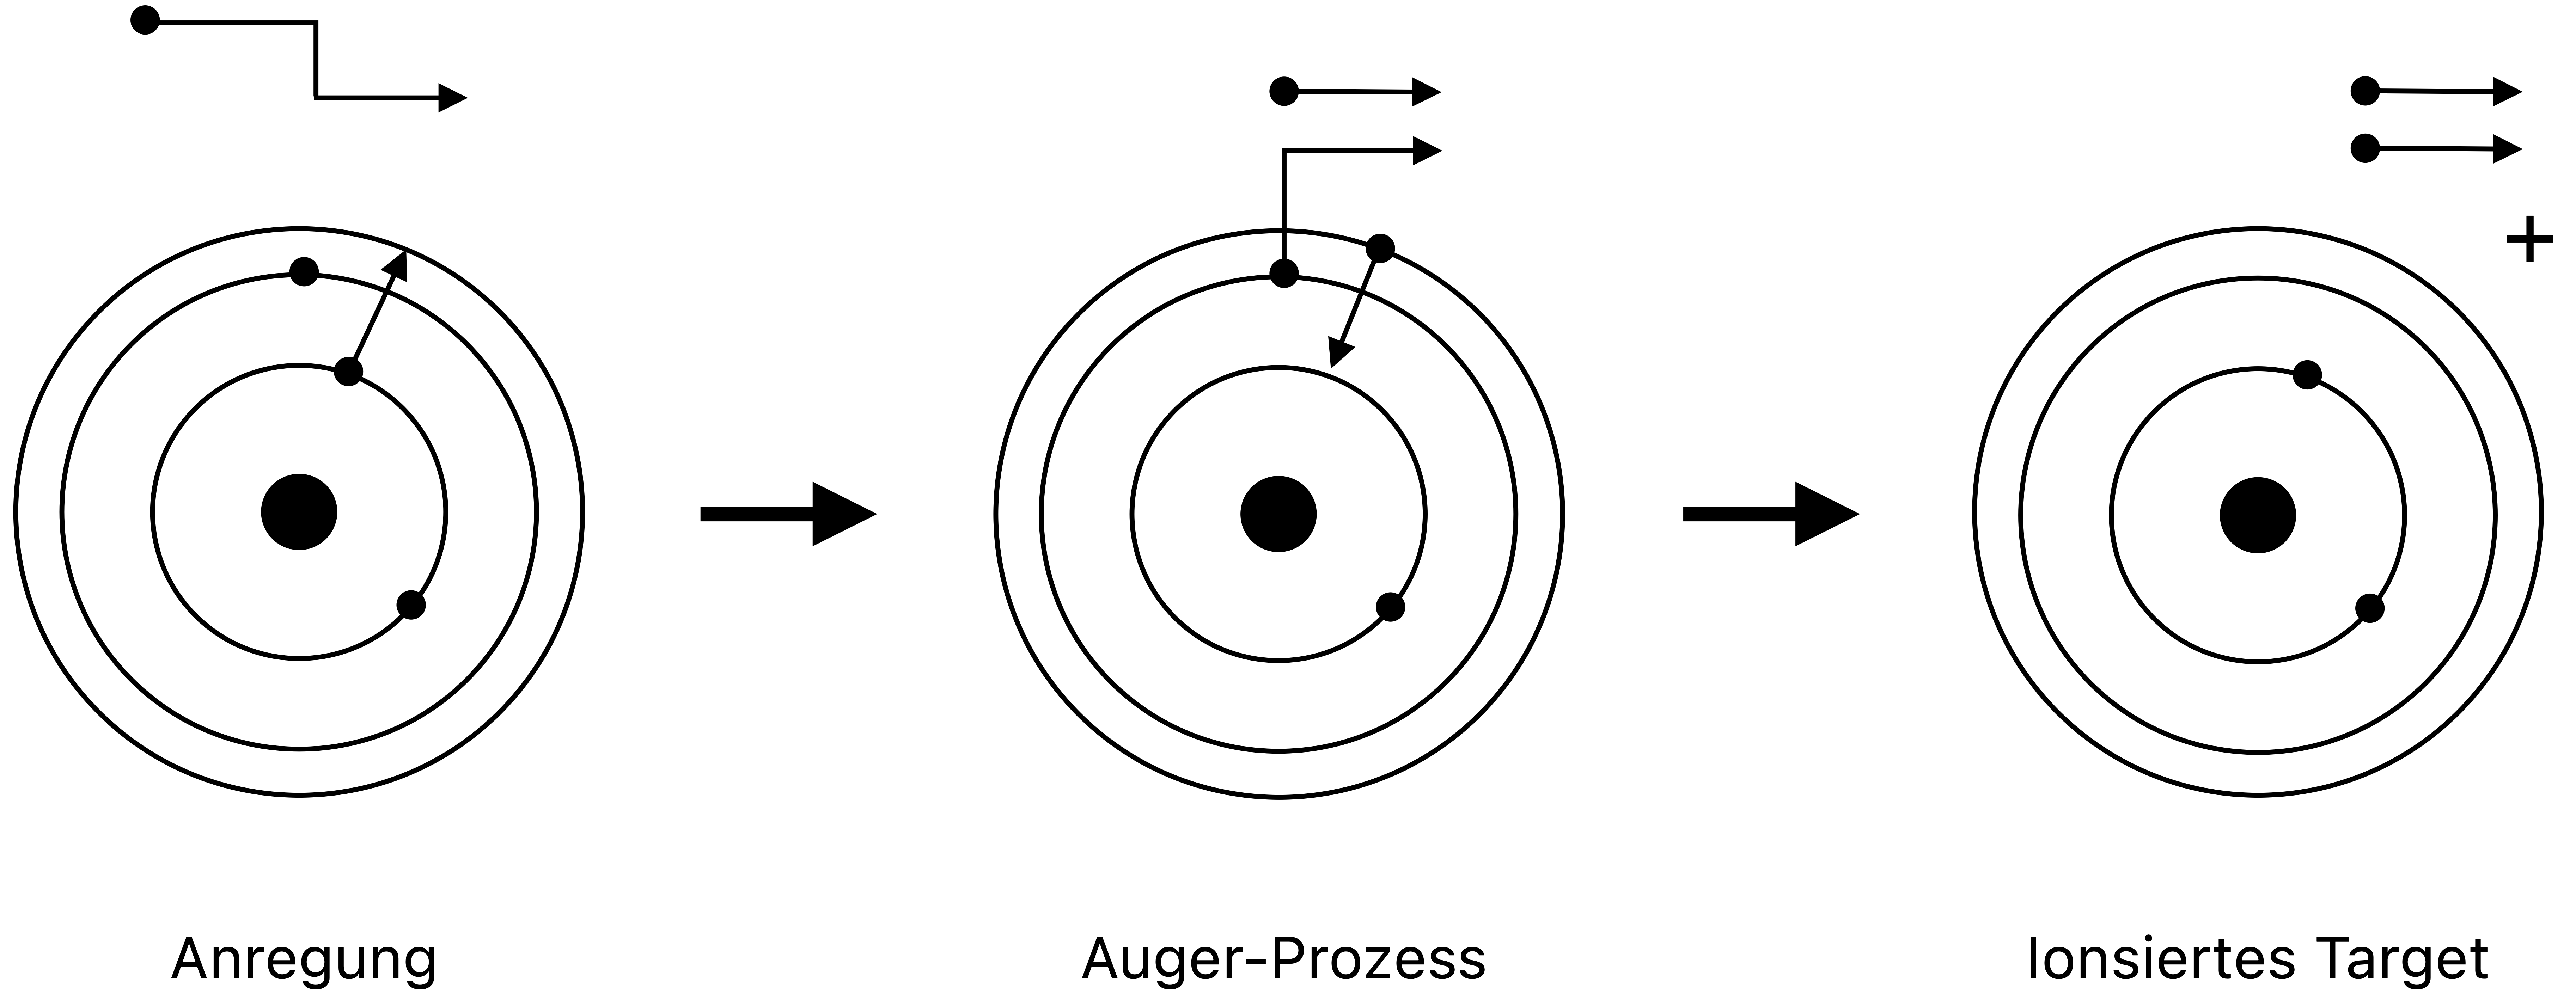
\includegraphics[width=.9\textwidth]{EA.png}
    \caption{Schematische Darstellung der Anregungs-Autoionisation für ein Atom.}
    \label{fig:EA}
\end{figure}
Weil bei der Anregungs-Autoionisation sowohl das Coloumb-Potential des Targets als auch die nötige Energie für die Anregung eines Elektrons überwunden werden müssen, tritt dieser Prozess erst bei höheren Energien auf. 

Es ist auch möglich eine Kombination aus DI und EA zu beobachten, bei der durch den Energieübertrag direkt ein Elektron aus einer inneren Schale herausgelöst wird und so das Target eine instabile Elektronenkonfiguration bekommt. Bei der folgenden Abregung kann es dann auch zum Auger-Prozess kommen. Mit steigender Energie des stoßenden Elektrons steigt die Wahrscheinlichkeit für mehrstufige Prozesse und es sind noch höhere Anregungen, die zu Mehrfachionisationen über Auger-Kaskaden führen, möglich.

Bei Molekülen kann es dazu kommen, dass das aus der Wechselwirkung resultierende ionisierte Molekül nicht stabil ist und es zur Dissoziation kommt oder das Molekül vom Stoß eines Elektrons mit hoher Energie direkt dissoziiert wird. Dabei werden häufig Ionen oder Radikale gebildet, es können aber auch neutrale Fragmente entstehen. Dieser Vorgang wird als Dissoziationsionisation (engl. \textit{dissociative ionisation}, auch DI aber im Folgenden als DIS) bezeichnet, wenn der Zerfall aufgrund von Ionisation stattfindet. Ein solcher Prozess kann durch eine der folgende Reaktionsgleichungen beschrieben werden:
\begin{equation}
    AB + e^- \rightarrow A^{+} + B + 2e^-
\end{equation}
\begin{equation}
    AB + e^- \rightarrow AB^* + e^- \rightarrow A^{+} + B + 2e^-.
\end{equation} 
Hierbei ist $AB$ das Molekül und $AB^*$ das angeregte Molekül.

Über eine Reihe von Stoßionisationen können komplexe Moleküle so in viele verschiedene, kleinere Fragmente zerfallen. Aufgrund dieser hohen Fragmentierung wird die Elektronenstoßionisation als eine \textit{harte} Ionisationsmethode bezeichnet.

\subsection{Resonante Prozesse}
Bei der Ionisation von Atomen und Molekülen kann auch ein resonanter Prozess einen Zwischenschritt darstellen. Dabei wird das Elektron vom Target eingefangen und verbleibt nicht im Kontinuum (freien Zustand). Man spricht von Resonanz, da die Energie des Elektrons genau einem quantiesierten Energieniveau entsprechen muss, um temporär gebunden zu werden. Der daraus entstehende Zustand des Targets ist mit hoher Wahrscheinlichkeit instabil und endet häufig in Autoionisation. Da Moleküle aufgrund ihrer zusätzlichen Freiheitsgrade (Rotation, Schwingung) und überlappenden Orbitalen mehr diskrete Energieniveaus haben, sind resonante Prozesse beim Stoß von Elektronen mit Molekülen häufiger. Das sorgt auch für zusätzliche Dissoziation und wird als dissioziative Elektronenanlagerung (engl. \textit{Dissociative Electron Attachment}, DEA) bezeichnet. Resonante Ionisationsprozesse treten allerdings besonders beim Stoß von Elektronen und Ionen auf, weil das positive Potential anziehend auf das Elektron wirkt und sind deswegen für die Ionisation von Atomen weniger wichtig.

\section{Ionisierungsquerschnitt}
Der Ionisierungsquerschnitt beschreibt, wie effektiv das Analytgas ionisiert werden kann. Der Querschnitt setzt sich dabei aus den einzelnen Querschnitten der verschiedenen, beschriebenen Ionisationsprozesse zusammen. Er hängt vor allem von der Energie und Anzahl der Elektronen, sowie der Dichte des Gases ab. Unter der Bedingung, dass nur sehr wenige der Elektronen eine Kollision mit einem Targetatom haben, kann der Stoßionisierungsquerschnitt wie folgt beschrieben werden:

\begin{equation}
    \sigma_{\text{i}} = \frac{N_{\text{i}}}{N_{\text{e}} \cdot n l}.
\end{equation}

$N_i$ ist dabei die Anzahl der erzeugten Ionen und $N_e$ die Anzahl der Elektronen. $n$ ist die Teilchendichte des Gases und $l$ die Länge der Strecke, die die Elektronen im Gas zurücklegen. Einfach hergeleitet werden kann diese Formel über die Wechselwirkungwahrscheinlichkeit $P$. Diese ist gleich dem Verhältnis der Anzahl der Stoßionisationen zur Anzahl der Elektronen wie auch dem Produkt aus der Teilchendichte, der zurückgelegten Strecke und dem Stoßionisierungsquerschnitt: 
\begin{equation}
    P = \frac{N_i}{N_e} = n \cdot l \cdot \sigma_i.
\end{equation}
Das später nur ein Teil der erzeugten Ionen von einem Detektor nachgewiesen werden kann, wird für $l$ nur der Durchmesser der aktiven Fläche des Detektors berücksichtigt. 

Um eine akkurate Aufnahme des Ionisierungsquerschnitts zu erhalten, müssen die Anzahlen der Elektronen und Ionen möglichst genau gemessen werden. Die Anzahl der Elektronen muss durch die Messung des tatsächlichen Elektronenstroms bestimmt werden. Wie in der Anlange von Straub, wird auch in dieser Arbeit ein Elektronenstrahl aus einer Elektronenkanone verwendet, welcher auf ein Ladungsmesser gezielt wird.

\section{Einzelstoßbedingung}